\section{向量组}

向量组要研究的问题很朴素：一组向量里，哪些是“多余”的？去掉多余的部分后，还剩几个真正独立的方向？把这些方向当作坐标系，同一个向量又该怎样读数？下面从具体的组合运算开始，一路走到正交基。

\subsection{线性组合与线性表出}

取两个平面向量
\[
\boldsymbol{\alpha}_1=(1,1)^{\mathrm T},\qquad \boldsymbol{\alpha}_2=(1,-1)^{\mathrm T}.
\]
用系数 $2$ 和 $1$ 把它们拼起来：
\[
2\boldsymbol{\alpha}_1+\boldsymbol{\alpha}_2
=(2,2)^{\mathrm T}+(1,-1)^{\mathrm T}=(3,1)^{\mathrm T}.
\]
结果仍是平面上的一个向量。改变系数，终点就跟着变；所有可能的终点构成这两个向量能“够得着”的范围。

\begin{mydef}{线性组合与线性表出}{linear-combination}
设 $\boldsymbol{\alpha}_1,\ldots,\boldsymbol{\alpha}_m$ 是 $n$ 维向量，$k_1,\ldots,k_m$ 是实数。向量
\[
k_1\boldsymbol{\alpha}_1+k_2\boldsymbol{\alpha}_2+\cdots+k_m\boldsymbol{\alpha}_m
\]
称为这组向量的一个\textbf{线性组合}，$k_i$ 称为组合系数。

若存在实数 $x_1,\ldots,x_m$ 使
\[
\boldsymbol{\beta}=x_1\boldsymbol{\alpha}_1+x_2\boldsymbol{\alpha}_2+\cdots+x_m\boldsymbol{\alpha}_m,
\]
就说 $\boldsymbol{\beta}$ 可由 $\boldsymbol{\alpha}_1,\ldots,\boldsymbol{\alpha}_m$ \textbf{线性表出}，$x_i$ 就是表出系数。系数允许为 $0$ 或负数，没有“必须取正”的限制。
\end{mydef}

把向量按列排成矩阵 $A=(\boldsymbol{\alpha}_1,\ldots,\boldsymbol{\alpha}_m)$，表出式就是线性方程组
\[
A\boldsymbol{x}=\boldsymbol{\beta},\qquad \boldsymbol{x}=(x_1,\ldots,x_m)^{\mathrm T}.
\]
所以“能否表出”等价于“方程组是否有解”。由线性方程组的理论，
\[
\boldsymbol{\beta}\ \text{可被表出}\iff \operatorname{rank}(A)=\operatorname{rank}(A\mid\boldsymbol{\beta}).
\]
若还有 $\operatorname{rank}(A)=m$（各列线性无关），则解唯一；若秩小于 $m$，表出方式不唯一，有无穷多组系数。

\begin{center}
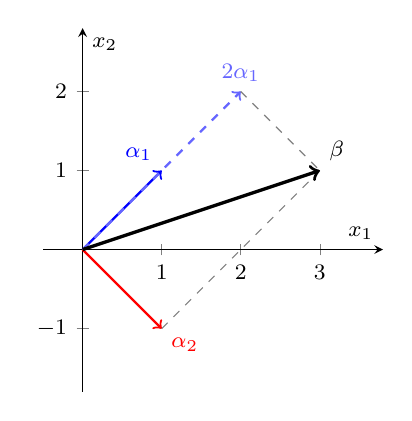
\begin{tikzpicture}
\begin{axis}[
  axis lines=center, axis equal image, clip=false,
  width=0.62\linewidth, height=6.2cm,
  xlabel={$x_1$}, ylabel={$x_2$},
  xmin=-0.5, xmax=3.8, ymin=-1.8, ymax=2.8,
  xtick={1,2,3}, ytick={-1,1,2},
  font=\footnotesize,
]
\draw[->,thick,blue] (axis cs:0,0) -- (axis cs:1,1);
\draw[->,thick,red]  (axis cs:0,0) -- (axis cs:1,-1);
\draw[->,thick,blue!60,dashed] (axis cs:0,0) -- (axis cs:2,2);
\draw[dashed,gray] (axis cs:2,2) -- (axis cs:3,1);
\draw[dashed,gray] (axis cs:1,-1) -- (axis cs:3,1);
\draw[->,very thick,black] (axis cs:0,0) -- (axis cs:3,1);
\node[blue,anchor=south east] at (axis cs:1,1) {$\boldsymbol{\alpha}_1$};
\node[red,anchor=north west] at (axis cs:1,-1) {$\boldsymbol{\alpha}_2$};
\node[blue!60,anchor=south] at (axis cs:2,2) {$2\boldsymbol{\alpha}_1$};
\node[black,anchor=south west] at (axis cs:3,1) {$\boldsymbol{\beta}$};
\end{axis}
\end{tikzpicture}
\end{center}

图中 $\boldsymbol{\beta}=2\boldsymbol{\alpha}_1+\boldsymbol{\alpha}_2$：先沿 $\boldsymbol{\alpha}_1$ 走两倍，再沿 $\boldsymbol{\alpha}_2$ 走一倍，两条虚线围成平行四边形，$\boldsymbol{\beta}$ 是它的对角线。只要两个向量不共线，改变两个系数就能到达平面上任意一点；一旦共线，无论怎么配系数，终点都只能留在同一条直线上。

\subsection{线性相关与线性无关}

看两个向量
\[
\boldsymbol{\alpha}_1=(1,2)^{\mathrm T},\qquad \boldsymbol{\alpha}_2=(2,4)^{\mathrm T}.
\]
显然 $\boldsymbol{\alpha}_2=2\boldsymbol{\alpha}_1$，移项得
\[
2\boldsymbol{\alpha}_1-\boldsymbol{\alpha}_2=\boldsymbol{0}.
\]
系数 $(2,-1)$ 不全为零，却把非零向量组合成了零向量。这说明 $\boldsymbol{\alpha}_2$ 没有提供新方向，是“多余”的。

\begin{mydef}{线性相关与线性无关}{linear-dependence}
对向量组 $\boldsymbol{\alpha}_1,\ldots,\boldsymbol{\alpha}_m$，若存在\textbf{不全为零}的实数 $k_1,\ldots,k_m$ 使
\[
k_1\boldsymbol{\alpha}_1+k_2\boldsymbol{\alpha}_2+\cdots+k_m\boldsymbol{\alpha}_m=\boldsymbol{0},
\]
则称该向量组\textbf{线性相关}。若上式只在 $k_1=\cdots=k_m=0$ 时成立，则称它\textbf{线性无关}。
\end{mydef}

“无关”不等于“任意两个都不成比例”这么简单，它要求整个组没有任何非平凡的零组合。单个向量 $\boldsymbol{\alpha}$ 线性相关当且仅当 $\boldsymbol{\alpha}=\boldsymbol{0}$；含有零向量的向量组一定线性相关，因为让零向量的系数取 $1$、其余取 $0$ 就得到零组合。

\begin{formula}{线性相关性的判定}{dependence-criteria}
设 $A=(\boldsymbol{\alpha}_1,\ldots,\boldsymbol{\alpha}_m)$ 是以这些向量为列的 $n\times m$ 矩阵。
\begin{enumerate}
  \item 齐次方程法：线性相关 $\iff$ $A\boldsymbol{x}=\boldsymbol{0}$ 有非零解；线性无关 $\iff$ 只有零解。
  \item 秩判别法：线性相关 $\iff$ $\operatorname{rank}(A)<m$；线性无关 $\iff$ $\operatorname{rank}(A)=m$。
  \item 行列式法（$m=n$）：$n$ 个 $n$ 维向量线性相关 $\iff$ $\det A=0$。
  \item 个数与维数：当 $m>n$ 时，$m$ 个 $n$ 维向量必定线性相关。因为 $n$ 维空间里最多只能放下 $n$ 个独立方向。
\end{enumerate}
\end{formula}

几何上，$\mathbb{R}^2$ 中两个向量线性相关就是共线，线性无关就是不共线；$\mathbb{R}^3$ 中三个向量线性相关就是共面，线性无关就是不共面。

\begin{center}
\begin{tikzpicture}[x=1.9cm,y=1.9cm,font=\footnotesize]
\begin{scope}
  \draw[->] (-1.5,0) -- (1.55,0) node[below] {$x_1$};
  \draw[->] (0,-1.5) -- (0,1.55) node[left] {$x_2$};
  \draw[->,thick,blue] (0,0) -- (1,0.8) node[above right] {$\boldsymbol{\alpha}_1$};
  \draw[->,thick,blue!60,dashed] (0,0) -- (-0.75,-0.6) node[below left] {$\boldsymbol{\alpha}_2$};
  \node at (0,1.9) {相关：共线};
\end{scope}
\begin{scope}[xshift=7.0cm]
  \draw[->] (-1.5,0) -- (1.55,0) node[below] {$x_1$};
  \draw[->] (0,-1.5) -- (0,1.55) node[left] {$x_2$};
  \draw[->,thick,blue] (0,0) -- (1,0.35) node[above right] {$\boldsymbol{\alpha}_1$};
  \draw[->,thick,red]  (0,0) -- (0.35,1) node[above right] {$\boldsymbol{\alpha}_2$};
  \node at (0,1.9) {无关：不共线};
\end{scope}
\end{tikzpicture}
\end{center}

左图两个箭头落在同一直线上，其中一个必然是另一个的倍数，存在非零系数把它们组合成零；右图两个箭头方向不同，要让组合等于零只能让两个系数都取零。

关于相关与无关，有几条经常直接拿来用的结论。

第一，部分相关则整体相关；反过来，整体无关则任何部分组都无关。原因是：部分组上的非平凡零组合，把其余向量的系数补成 $0$，就成了整个组的非平凡零组合。

第二，设 $\boldsymbol{\alpha}_1,\ldots,\boldsymbol{\alpha}_m$ 线性无关，而添上 $\boldsymbol{\beta}$ 后变为线性相关，则 $\boldsymbol{\beta}$ 可由原组表出，且表出方式唯一。证明很短：相关给出
\[
k_1\boldsymbol{\alpha}_1+\cdots+k_m\boldsymbol{\alpha}_m+k\boldsymbol{\beta}=\boldsymbol{0},
\]
其中系数不全为零。若 $k=0$，则原组自己就有非平凡零组合，与无关矛盾，所以 $k\neq0$，解出 $\boldsymbol{\beta}$ 即可。唯一性来自：两种表出相减，会得到原组的一个零组合，系数只能全为零。

第三，无关组添上一个“表不出来的向量”，得到的仍是无关组。这条结论说明无关组可以不断扩充，直到张满整个空间。

第四，若 $\boldsymbol{\alpha}_1,\ldots,\boldsymbol{\alpha}_r$ 线性无关，且每个 $\boldsymbol{\alpha}_i$ 都能由 $\boldsymbol{\beta}_1,\ldots,\boldsymbol{\beta}_s$ 表出，则 $r\le s$。直观上，$s$ 个向量最多提供 $s$ 个独立方向，装不下 $r$ 个独立方向。这条“数个数”的事实后面会用来证明秩与极大无关组的大小无关。

还要注意：线性相关只保证“至少有一个”向量能由其余向量表出，不保证每一个都能。例如
\[
\boldsymbol{\alpha}_1=(1,0)^{\mathrm T},\quad
\boldsymbol{\alpha}_2=(2,0)^{\mathrm T},\quad
\boldsymbol{\alpha}_3=(0,1)^{\mathrm T}
\]
线性相关，但 $\boldsymbol{\alpha}_3$ 无法由前两个向量表出，因为前两个向量张成的只是一条 $x$ 轴。

\subsection{极大无关组与秩}

在 $\mathbb{R}^3$ 中取四个向量
\[
\boldsymbol{\alpha}_1=\begin{pmatrix}1\\0\\1\end{pmatrix},\quad
\boldsymbol{\alpha}_2=\begin{pmatrix}0\\1\\1\end{pmatrix},\quad
\boldsymbol{\alpha}_3=\begin{pmatrix}1\\1\\2\end{pmatrix},\quad
\boldsymbol{\alpha}_4=\begin{pmatrix}1\\0\\0\end{pmatrix}.
\]
直接观察发现 $\boldsymbol{\alpha}_3=\boldsymbol{\alpha}_1+\boldsymbol{\alpha}_2$，所以 $\boldsymbol{\alpha}_3$ 没有带来新方向。把它去掉，剩下三个向量
\[
\det(\boldsymbol{\alpha}_1,\boldsymbol{\alpha}_2,\boldsymbol{\alpha}_4)
=\begin{vmatrix}1&0&1\\0&1&0\\1&1&0\end{vmatrix}=-1\neq0,
\]
线性无关，而且 $\boldsymbol{\alpha}_3$ 已经能用它们表出。因此 $\{\boldsymbol{\alpha}_1,\boldsymbol{\alpha}_2,\boldsymbol{\alpha}_4\}$ 是这组向量里“不多不少”的一部分。

\begin{center}
\begin{tikzpicture}[font=\footnotesize,x=1.1cm,y=1.1cm]
% 平面 span{α1, α2}
\fill[blue!8] (0,0) -- (4.2,-0.5) -- (5.4,1.4) -- (1.2,1.9) -- cycle;
\draw[blue!45] (0,0) -- (4.2,-0.5) -- (5.4,1.4) -- (1.2,1.9) -- cycle;
% 平面内的三个向量
\draw[->,thick,red] (0,0) -- (4.2,-0.5) node[below] {$\boldsymbol{\alpha}_1$};
\draw[->,thick,green!50!black] (0,0) -- (1.2,1.9) node[above left] {$\boldsymbol{\alpha}_2$};
\draw[->,thick,orange] (0,0) -- (5.4,1.4) node[above right] {$\boldsymbol{\alpha}_3$};
% 指向平面外的向量
\draw[->,very thick,blue] (0,0) -- (0,3.0) node[right] {$\boldsymbol{\alpha}_4$\ 平面外};
\node[blue!55!black] at (3.4,0.85) {$\operatorname{span}\{\boldsymbol{\alpha}_1,\boldsymbol{\alpha}_2\}$};
\end{tikzpicture}
\end{center}

图中 $\boldsymbol{\alpha}_1,\boldsymbol{\alpha}_2$ 张成一个平面，$\boldsymbol{\alpha}_3$ 仍落在这个平面内，所以添上它不增加维数。$\boldsymbol{\alpha}_4$ 指向平面外，张成空间从二维升到三维，秩也从 $2$ 变成 $3$。若只有前两个向量，极大无关组就是它俩；加入 $\boldsymbol{\alpha}_4$ 后，极大无关组需要三个向量。

\begin{mydef}{极大线性无关组与秩}{maximal-independent-set}
设 $S=\{\boldsymbol{\alpha}_1,\ldots,\boldsymbol{\alpha}_m\}$。若它的一个部分组 $\boldsymbol{\alpha}_{i_1},\ldots,\boldsymbol{\alpha}_{i_r}$ 满足
\begin{enumerate}
  \item 自身线性无关；
  \item 从 $S$ 中再任取一个剩余向量添进去，所得向量组都线性相关，
\end{enumerate}
则称它为 $S$ 的一个\textbf{极大线性无关组}，简称极大无关组。

极大无关组所含向量的个数称为向量组 $S$ 的\textbf{秩}，记作 $\operatorname{rank}(S)$。只含零向量的向量组规定秩为 $0$。
\end{mydef}

定义中的第二条也可以换成“原向量组中每个向量都能由这 $r$ 个向量表出”。两种说法等价：若每个向量都能被表出，再添任何一个都会变成相关；反之，若添任何一个都相关，由上一节的结论，每个剩余向量都能被表出。

极大无关组不一定唯一。上例中 $\{\boldsymbol{\alpha}_1,\boldsymbol{\alpha}_2,\boldsymbol{\alpha}_4\}$ 是一个，$\{\boldsymbol{\alpha}_2,\boldsymbol{\alpha}_3,\boldsymbol{\alpha}_4\}$ 也是一个，因为 $\boldsymbol{\alpha}_3=\boldsymbol{\alpha}_1+\boldsymbol{\alpha}_2$ 同样能顶替 $\boldsymbol{\alpha}_1$。但所有极大无关组含有的向量个数相同，这个公共个数就是秩。设两个极大无关组分别含 $r$ 和 $t$ 个向量；它们都与原向量组等价，因而彼此可以互相表出。用前面的替换定理分别比较，得到 $r\le t$ 和 $t\le r$，所以 $r=t$。

由此得到几条常用性质：
\begin{itemize}
  \item 向量组与它的任意一个极大无关组等价，也就是可以互相线性表出；
  \item $\operatorname{rank}(S)=\dim\operatorname{span}(S)$，秩就是这组向量张成的子空间的维数；
  \item $0\le \operatorname{rank}(S)\le \min\{m,n\}$，其中 $m$ 是向量个数，$n$ 是向量维数；
  \item 向量组线性无关 $\iff$ 秩等于向量个数 $m$；
  \item 往向量组里添向量，秩不会减小；删去向量，秩不会增大。
\end{itemize}

把向量按列排成矩阵，行变换后的主元列如下：

\begin{center}
\begin{tikzpicture}[font=\footnotesize,x=1.2cm,y=0.68cm]
% 第 3 列标灰：它不是主元列
\fill[gray!18] (2,0) rectangle (3,-3);
% 主元格
\fill[blue!15] (0,0) rectangle (1,-1);
\fill[blue!15] (1,-1) rectangle (2,-2);
\fill[blue!15] (3,-2) rectangle (4,-3);
\draw[gray!60] (0,0) grid (4,-3);
\node at (0.5,0.42) {$\boldsymbol{\alpha}_1$};
\node at (1.5,0.42) {$\boldsymbol{\alpha}_2$};
\node at (2.5,0.42) {$\boldsymbol{\alpha}_3$};
\node at (3.5,0.42) {$\boldsymbol{\alpha}_4$};
\node at (0.5,-0.5) {$1$};
\node at (1.5,-0.5) {$0$};
\node at (2.5,-0.5) {$1$};
\node at (3.5,-0.5) {$0$};
\node at (0.5,-1.5) {$0$};
\node at (1.5,-1.5) {$1$};
\node at (2.5,-1.5) {$1$};
\node at (3.5,-1.5) {$0$};
\node at (0.5,-2.5) {$0$};
\node at (1.5,-2.5) {$0$};
\node at (2.5,-2.5) {$0$};
\node at (3.5,-2.5) {$1$};
\node[anchor=north] at (2,-3.25) {第 3 列 $=$ 第 1 列 $+$ 第 2 列};
\node[anchor=north] at (2,-3.95) {故 $\boldsymbol{\alpha}_3=\boldsymbol{\alpha}_1+\boldsymbol{\alpha}_2$};
\end{tikzpicture}

\vspace{0.2em}
{\footnotesize 行最简形里的主元列：蓝色格子是主元，其列标对应的原向量构成一个极大无关组；灰色第 3 列可由主元列表出。}
\end{center}

求极大无关组和秩，不必真的去试遍所有部分组。把向量按列排成矩阵 $A$，只做初等行变换，化成行阶梯形或行最简形。行变换相当于在左边乘一个可逆矩阵 $P$，而
\[
A\boldsymbol{x}=\boldsymbol{0}\iff PA\boldsymbol{x}=\boldsymbol{0},
\]
所以列与列之间的线性关系完全不变。化成行最简形后，主元所在列对应的那些\textbf{原向量}就构成一个极大无关组；主元个数就是秩。非主元列的系数可以直接从行最简形读出，用来表出其余向量。

上例的矩阵正是
\[
A=(\boldsymbol{\alpha}_1,\boldsymbol{\alpha}_2,\boldsymbol{\alpha}_3,\boldsymbol{\alpha}_4)
=\begin{pmatrix}
1&0&1&1\\
0&1&1&0\\
1&1&2&0
\end{pmatrix}
\xrightarrow{r_3-r_1-r_2}
\begin{pmatrix}
1&0&1&1\\
0&1&1&0\\
0&0&0&-1
\end{pmatrix}
\]
再把第三行乘 $-1$，用它消去第一行第四列的 $1$，得到行最简形
\[
\begin{pmatrix}
1&0&1&0\\
0&1&1&0\\
0&0&0&1
\end{pmatrix}.
\]
主元在第 $1,2,4$ 列，所以 $\{\boldsymbol{\alpha}_1,\boldsymbol{\alpha}_2,\boldsymbol{\alpha}_4\}$ 是极大无关组，秩为 $3$。第 $3$ 列是 $(1,1,0)^{\mathrm T}$，直接读出
\[
\boldsymbol{\alpha}_3=\boldsymbol{\alpha}_1+\boldsymbol{\alpha}_2.
\]
注意，行最简形里的列已经不是原来的 $\boldsymbol{\alpha}_i$ 了，但列之间的系数关系保持不变；最后写表出式时，要用原向量。

\subsection{基、坐标与基变换}

同一个向量，换一组“尺子”去量，读数会变。取
\[
\boldsymbol{\alpha}=(3,1)^{\mathrm T},\qquad
\boldsymbol{\varepsilon}'_1=(1,1)^{\mathrm T},\qquad
\boldsymbol{\varepsilon}'_2=(1,-1)^{\mathrm T}.
\]
直接验证
\[
2\boldsymbol{\varepsilon}'_1+1\boldsymbol{\varepsilon}'_2=(2,2)^{\mathrm T}+(1,-1)^{\mathrm T}=(3,1)^{\mathrm T}=\boldsymbol{\alpha}.
\]
所以在标准基 $\boldsymbol{e}_1=(1,0)^{\mathrm T},\boldsymbol{e}_2=(0,1)^{\mathrm T}$ 下，$\boldsymbol{\alpha}$ 的坐标是 $(3,1)^{\mathrm T}$；换到 $\boldsymbol{\varepsilon}'_1,\boldsymbol{\varepsilon}'_2$ 下，坐标变成 $(2,1)^{\mathrm T}$。向量本身没动，变的只是描述方式。

\begin{mydef}{基、维数与坐标}{basis-and-coordinates}
设 $V$ 是一个向量空间。若 $V$ 中的向量组 $\boldsymbol{\varepsilon}_1,\ldots,\boldsymbol{\varepsilon}_n$ 线性无关，且 $V$ 中每个向量都能由它们线性表出，则称它们为 $V$ 的一组\textbf{基}，$n$ 称为 $V$ 的\textbf{维数}，记作 $\dim V$。零空间 $\{\boldsymbol{0}\}$ 的维数规定为 $0$。

取定一组基后，任意 $\boldsymbol{\alpha}\in V$ 的表出系数是唯一的：
\[
\boldsymbol{\alpha}=x_1\boldsymbol{\varepsilon}_1+\cdots+x_n\boldsymbol{\varepsilon}_n,
\]
列向量 $(x_1,\ldots,x_n)^{\mathrm T}$ 称为 $\boldsymbol{\alpha}$ 在这组基下的\textbf{坐标}。
\end{mydef}

坐标的唯一性来自无关性：若有两组系数，相减就得到基向量的一个零组合，系数只能全为零。

\begin{center}
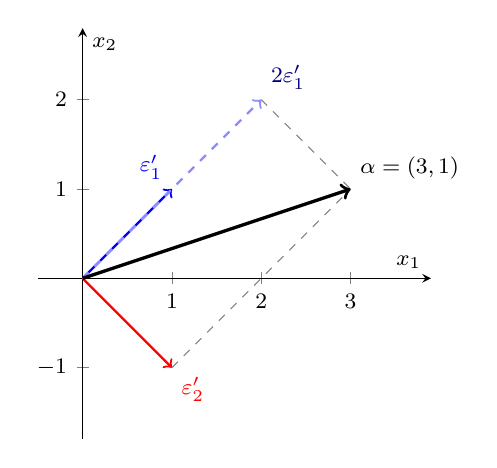
\begin{tikzpicture}
\begin{axis}[
  axis lines=center, axis equal image, clip=false,
  width=0.70\linewidth, height=6.8cm,
  xlabel={$x_1$}, ylabel={$x_2$},
  xmin=-0.5, xmax=3.9, ymin=-1.8, ymax=2.8,
  xtick={1,2,3}, ytick={-1,1,2},
  font=\footnotesize,
]
\draw[->,thick,blue] (axis cs:0,0) -- (axis cs:1,1);
\draw[->,thick,red]  (axis cs:0,0) -- (axis cs:1,-1);
\draw[->,blue!45,thick,dashed] (axis cs:0,0) -- (axis cs:2,2);
\draw[dashed,gray] (axis cs:2,2) -- (axis cs:3,1);
\draw[dashed,gray] (axis cs:1,-1) -- (axis cs:3,1);
\draw[->,very thick,black] (axis cs:0,0) -- (axis cs:3,1);
\node[blue,anchor=south east] at (axis cs:1,1) {$\boldsymbol{\varepsilon}'_1$};
\node[red,anchor=north west] at (axis cs:1,-1) {$\boldsymbol{\varepsilon}'_2$};
\node[blue!50!black,anchor=south west] at (axis cs:2,2) {$2\boldsymbol{\varepsilon}'_1$};
\node[black,anchor=south west] at (axis cs:3,1) {$\boldsymbol{\alpha}=(3,1)$};
\end{axis}
\end{tikzpicture}
\end{center}

图中实线箭头是新基的两个向量，虚线平行四边形说明 $\boldsymbol{\alpha}$ 要沿 $\boldsymbol{\varepsilon}'_1$ 走两格、沿 $\boldsymbol{\varepsilon}'_2$ 走一格。于是同一终点在旧基下读作 $(3,1)$，在新基下读作 $(2,1)$。

在 $\mathbb{R}^n$ 中，$\boldsymbol{e}_1,\ldots,\boldsymbol{e}_n$（第 $i$ 个位置为 $1$、其余为 $0$）构成\textbf{标准基}。向量 $(a_1,\ldots,a_n)^{\mathrm T}$ 在标准基下的坐标就是它的分量本身。判断 $\mathbb{R}^n$ 中 $n$ 个向量是否构成基，只需看以它们为列的矩阵行列式是否非零；非零则线性无关，而 $n$ 个无关向量自动张满 $\mathbb{R}^n$。

两组基之间用一个矩阵联系。设旧基为 $\boldsymbol{\varepsilon}_1,\ldots,\boldsymbol{\varepsilon}_n$，新基为 $\boldsymbol{\varepsilon}'_1,\ldots,\boldsymbol{\varepsilon}'_n$。把新基向量用旧基表出：
\[
(\boldsymbol{\varepsilon}'_1,\ldots,\boldsymbol{\varepsilon}'_n)
=(\boldsymbol{\varepsilon}_1,\ldots,\boldsymbol{\varepsilon}_n)P.
\]
矩阵 $P$ 称为从旧基到新基的\textbf{过渡矩阵}。它的第 $j$ 列就是 $\boldsymbol{\varepsilon}'_j$ 在旧基下的坐标。由于新旧两组都是基，$P$ 一定可逆。

若同一个向量在旧基下的坐标为 $\boldsymbol{x}$，在新基下的坐标为 $\boldsymbol{x}'$，则
\[
\boldsymbol{\alpha}=(\boldsymbol{\varepsilon}_1,\ldots,\boldsymbol{\varepsilon}_n)\boldsymbol{x}
=(\boldsymbol{\varepsilon}'_1,\ldots,\boldsymbol{\varepsilon}'_n)\boldsymbol{x}'
=(\boldsymbol{\varepsilon}_1,\ldots,\boldsymbol{\varepsilon}_n)P\boldsymbol{x}'.
\]
由坐标唯一性，
\[
\boldsymbol{x}=P\boldsymbol{x}',\qquad\text{即}\qquad \boldsymbol{x}'=P^{-1}\boldsymbol{x}.
\]
方向不要弄反：$P$ 把新坐标送回旧坐标；要从旧坐标求新坐标，得乘 $P^{-1}$。

用上面的例子算一遍。旧基是标准基，所以
\[
P=\begin{pmatrix}1&1\\1&-1\end{pmatrix},\qquad
P^{-1}=\frac{1}{-2}\begin{pmatrix}-1&-1\\-1&1\end{pmatrix}
=\begin{pmatrix}\frac12&\frac12\\[2pt]\frac12&-\frac12\end{pmatrix}.
\]
于是
\[
\boldsymbol{x}'=P^{-1}\begin{pmatrix}3\\1\end{pmatrix}
=\begin{pmatrix}2\\1\end{pmatrix},
\]
与直接观察一致。若再从新基换到第三组基，过渡矩阵按顺序相乘：旧到新用 $P$，新到第三组用 $Q$，则旧到第三组用 $PQ$。反向的过渡矩阵就是 $P^{-1}$。

\subsection{内积、正交基与 Schmidt 正交化}

坐标一般要解方程组才能得到，但如果基向量两两垂直，坐标可以直接用内积算出来。先看反例。取基
\[
\boldsymbol{\varepsilon}_1=(1,1)^{\mathrm T},\qquad \boldsymbol{\varepsilon}_2=(1,0)^{\mathrm T},
\]
它们不垂直。向量 $\boldsymbol{\alpha}=(3,1)^{\mathrm T}$ 的坐标是 $(1,2)^{\mathrm T}$，因为
\[
1\cdot(1,1)^{\mathrm T}+2\cdot(1,0)^{\mathrm T}=(3,1)^{\mathrm T}.
\]
但
\[
\frac{(\boldsymbol{\alpha},\boldsymbol{\varepsilon}_1)}{(\boldsymbol{\varepsilon}_1,\boldsymbol{\varepsilon}_1)}
=\frac{4}{2}=2\neq 1,
\]
直接拿内积作商并得不到第一个坐标。原因是 $\boldsymbol{\varepsilon}_2$ 在 $\boldsymbol{\varepsilon}_1$ 上有分量，内积把这份“串扰”也算了进去。

回忆内积
\[
(\boldsymbol{\alpha},\boldsymbol{\beta})=\boldsymbol{\alpha}^{\mathrm T}\boldsymbol{\beta}
=\sum_{i=1}^n a_i b_i,
\]
它是对称、线性且正定的。向量长度 $\lVert\boldsymbol{\alpha}\rVert=\sqrt{(\boldsymbol{\alpha},\boldsymbol{\alpha})}$；内积为零时称两个向量\textbf{正交}。一组两两正交的非零向量一定线性无关：若 $\sum k_i\boldsymbol{\beta}_i=\boldsymbol{0}$，两边与 $\boldsymbol{\beta}_j$ 作内积，只剩 $k_j(\boldsymbol{\beta}_j,\boldsymbol{\beta}_j)=0$，故 $k_j=0$。

若 $\boldsymbol{\varepsilon}_1,\ldots,\boldsymbol{\varepsilon}_n$ 是一组正交基（两两内积为零），则
\[
\boldsymbol{\alpha}=\sum_{i=1}^n
\frac{(\boldsymbol{\alpha},\boldsymbol{\varepsilon}_i)}{(\boldsymbol{\varepsilon}_i,\boldsymbol{\varepsilon}_i)}
\boldsymbol{\varepsilon}_i.
\]
推导只需两边与 $\boldsymbol{\varepsilon}_j$ 作内积：正交性让所有 $i\neq j$ 的项消失，立刻解出系数。若基还是标准正交基（每个向量长度为 $1$），公式简化为 $x_i=(\boldsymbol{\alpha},\boldsymbol{\varepsilon}_i)$，坐标就是投影长度。

实际拿到的一组基通常不正交。Schmidt 正交化的做法是逐个“扣掉投影”，把无关组改造成正交组。设 $\boldsymbol{\alpha}_1,\ldots,\boldsymbol{\alpha}_m$ 线性无关，令
\[
\boldsymbol{\beta}_1=\boldsymbol{\alpha}_1,\qquad
\boldsymbol{\beta}_k=\boldsymbol{\alpha}_k-\sum_{i=1}^{k-1}
\frac{(\boldsymbol{\alpha}_k,\boldsymbol{\beta}_i)}{(\boldsymbol{\beta}_i,\boldsymbol{\beta}_i)}
\boldsymbol{\beta}_i,\quad k=2,\ldots,m.
\]
每一步都用 $\boldsymbol{\alpha}_k$ 减去它在已有各方向上的投影，剩下的 $\boldsymbol{\beta}_k$ 就与前面所有 $\boldsymbol{\beta}_i$ 垂直。由于 $\boldsymbol{\alpha}_k$ 不能由前面的向量表出，减完之后不会变成零向量。最后令
\[
\boldsymbol{e}_i=\frac{\boldsymbol{\beta}_i}{\lVert\boldsymbol{\beta}_i\rVert},
\]
就得到标准正交基。正交化不改变张成的子空间，所以 $(\boldsymbol{\beta}_1,\ldots,\boldsymbol{\beta}_m)$ 与 $(\boldsymbol{\alpha}_1,\ldots,\boldsymbol{\alpha}_m)$ 张成同一个空间。

\begin{center}
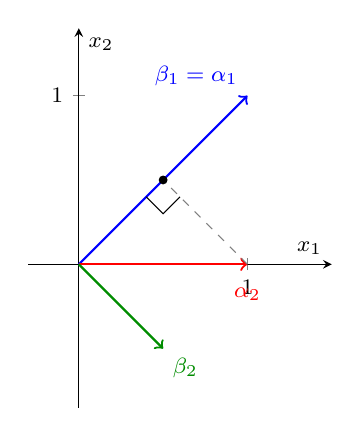
\begin{tikzpicture}
\begin{axis}[
  axis lines=center, axis equal image, clip=false,
  width=0.62\linewidth, height=6.4cm,
  xlabel={$x_1$}, ylabel={$x_2$},
  xmin=-0.3, xmax=1.5, ymin=-0.85, ymax=1.4,
  xtick={1}, ytick={1},
  font=\footnotesize,
]
\draw[->,thick,blue] (axis cs:0,0) -- (axis cs:1,1);
\draw[->,thick,red]  (axis cs:0,0) -- (axis cs:1,0);
\draw[->,thick,green!55!black] (axis cs:0,0) -- (axis cs:0.5,-0.5);
\draw[dashed,gray] (axis cs:1,0) -- (axis cs:0.5,0.5);
\fill (axis cs:0.5,0.5) circle (1.6pt);
\draw (axis cs:0.40,0.40) -- (axis cs:0.50,0.30) -- (axis cs:0.60,0.40);
\node[blue,anchor=south east] at (axis cs:1,1) {$\boldsymbol{\beta}_1=\boldsymbol{\alpha}_1$};
\node[red,anchor=north] at (axis cs:1,-0.08) {$\boldsymbol{\alpha}_2$};
\node[green!55!black,anchor=north west] at (axis cs:0.5,-0.5) {$\boldsymbol{\beta}_2$};
\end{axis}
\end{tikzpicture}
\end{center}

图中 $\boldsymbol{\alpha}_2$ 先投影到 $\boldsymbol{\beta}_1$ 上，得到虚线落点；再从 $\boldsymbol{\alpha}_2$ 减去这段投影，剩下的绿色箭头 $\boldsymbol{\beta}_2$ 与 $\boldsymbol{\beta}_1$ 垂直（小方块标出直角）。如果先处理 $\boldsymbol{\alpha}_1$，它本身就是 $\boldsymbol{\beta}_1$；处理第二个向量时只需扣掉一个投影，向量更多时就逐个扣掉所有已有方向上的投影。

用前面的例子走一遍。取 $\boldsymbol{\alpha}_1=(1,1)^{\mathrm T}$，$\boldsymbol{\alpha}_2=(1,0)^{\mathrm T}$，则
\[
\boldsymbol{\beta}_1=(1,1)^{\mathrm T},\qquad
(\boldsymbol{\alpha}_2,\boldsymbol{\beta}_1)=1,\quad
(\boldsymbol{\beta}_1,\boldsymbol{\beta}_1)=2,
\]
所以
\[
\boldsymbol{\beta}_2=(1,0)^{\mathrm T}-\frac12(1,1)^{\mathrm T}
=\left(\frac12,-\frac12\right)^{\mathrm T}.
\]
单位化后
\[
\boldsymbol{e}_1=\frac{1}{\sqrt2}\begin{pmatrix}1\\1\end{pmatrix},\qquad
\boldsymbol{e}_2=\frac{1}{\sqrt2}\begin{pmatrix}1\\-1\end{pmatrix}.
\]
这正是上一节用过的新基方向，只是长度被缩放到了 $1$。

现在再算 $\boldsymbol{\alpha}=(3,1)^{\mathrm T}$ 在这组标准正交基下的坐标：
\[
(\boldsymbol{\alpha},\boldsymbol{e}_1)=\frac{4}{\sqrt2}=2\sqrt2,\qquad
(\boldsymbol{\alpha},\boldsymbol{e}_2)=\frac{2}{\sqrt2}=\sqrt2.
\]
坐标为 $(2\sqrt2,\sqrt2)^{\mathrm T}$。它与上一节的 $(2,1)^{\mathrm T}$ 不相等，因为这里的基向量长度是 $1$，而上一节的基向量长度是 $\sqrt2$；把 $(2,1)$ 的每个分量乘以 $\sqrt2$，正好得到 $(2\sqrt2,\sqrt2)$。

把 $\boldsymbol{\alpha}_1,\ldots,\boldsymbol{\alpha}_n$ 按列排成矩阵 $A$，Schmidt 正交化的结果可以写成矩阵分解
\[
A=QR,
\]
其中 $Q$ 的列是标准正交基，$R$ 是上三角矩阵，对角元为 $\lVert\boldsymbol{\beta}_i\rVert$。这个分解要求 $A$ 的列线性无关，否则某一步会出现零向量，$R$ 不可逆。

\section{习题}

\subsection{本章速览}

\begin{itemize}
    \item \textbf{线性相关}：存在不全为零的系数 $k_1,\ldots,k_m$ 使 $k_1\boldsymbol{\alpha}_1+\cdots+k_m\boldsymbol{\alpha}_m=\boldsymbol{0}$。若只有全零系数才行，就叫\textbf{线性无关}。
    \item 把向量按列排成矩阵 $A$：线性相关 $\Leftrightarrow$ $A\boldsymbol{x}=\boldsymbol{0}$ 有非零解 $\Leftrightarrow$ $\operatorname{rank}(A)<m$（$m$ 为向量个数）；线性无关 $\Leftrightarrow$ $\operatorname{rank}(A)=m$。当 $m=n$ 时，直接看行列式是否为零。
    \item \textbf{极大无关组}：组内线性无关，且再添组内剩余的任何一个向量都线性相关。它与原向量组等价，所含向量个数就是\textbf{秩}。求法：按列排矩阵，行变换化行阶梯形，主元所在列对应的原向量即为一组极大无关组。
    \item \textbf{基与坐标}：基是“线性无关且能表出空间中每个向量”的向量组；基中向量个数为维数。向量在一组基下的坐标就是表出系数，坐标随基改变，但向量本身不变。
    \item \textbf{Schmidt 正交化}：$\boldsymbol{\beta}_1=\boldsymbol{\alpha}_1$，$\boldsymbol{\beta}_k=\boldsymbol{\alpha}_k-\sum_{i=1}^{k-1}\dfrac{\boldsymbol{\alpha}_k\cdot\boldsymbol{\beta}_i}{\boldsymbol{\beta}_i\cdot\boldsymbol{\beta}_i}\boldsymbol{\beta}_i$，再令 $\boldsymbol{e}_i=\dfrac{\boldsymbol{\beta}_i}{\|\boldsymbol{\beta}_i\|}$。在正交基下，坐标可用内积直接算：$x_i=\dfrac{\boldsymbol{\alpha}\cdot\boldsymbol{\varepsilon}_i}{\boldsymbol{\varepsilon}_i\cdot\boldsymbol{\varepsilon}_i}$。
\end{itemize}

\subsection{基础过关题}

\textbf{1.} 设 $\boldsymbol{\alpha}_1,\boldsymbol{\alpha}_2,\boldsymbol{\alpha}_3$ 线性无关，则下列向量组中线性无关的是（\quad）。
\begin{enumerate}[label=(\Alph*)]
    \item $\boldsymbol{\alpha}_1-\boldsymbol{\alpha}_2,\ \boldsymbol{\alpha}_2-\boldsymbol{\alpha}_3,\ \boldsymbol{\alpha}_3-\boldsymbol{\alpha}_1$
    \item $\boldsymbol{\alpha}_1+\boldsymbol{\alpha}_2,\ \boldsymbol{\alpha}_2+\boldsymbol{\alpha}_3,\ \boldsymbol{\alpha}_1-\boldsymbol{\alpha}_3$
    \item $\boldsymbol{\alpha}_1+2\boldsymbol{\alpha}_2,\ \boldsymbol{\alpha}_2+3\boldsymbol{\alpha}_3,\ 3\boldsymbol{\alpha}_3+\boldsymbol{\alpha}_1$
    \item $\boldsymbol{\alpha}_1+\boldsymbol{\alpha}_2+\boldsymbol{\alpha}_3,\ \boldsymbol{\alpha}_1-\boldsymbol{\alpha}_2+\boldsymbol{\alpha}_3,\ 2\boldsymbol{\alpha}_1+2\boldsymbol{\alpha}_3$
\end{enumerate}

\ifshowsolutions%
\boxed{\textbf{解}}\quad
\textbf{思路：} 因为 $\boldsymbol{\alpha}_1,\boldsymbol{\alpha}_2,\boldsymbol{\alpha}_3$ 线性无关，可以把它们临时当作一组“基”。把每个新向量在这组基下的坐标写成列，得到系数矩阵 $C$。新向量组线性无关当且仅当 $C$ 的列向量线性无关，即 $\det C\neq 0$。

设新向量组为 $\boldsymbol{\gamma}_1,\boldsymbol{\gamma}_2,\boldsymbol{\gamma}_3$，且 $\boldsymbol{\gamma}_j=\sum_{i=1}^{3}c_{ij}\boldsymbol{\alpha}_i$，则
\[
k_1\boldsymbol{\gamma}_1+k_2\boldsymbol{\gamma}_2+k_3\boldsymbol{\gamma}_3
=\sum_{i=1}^{3}\Bigl(\sum_{j=1}^{3}c_{ij}k_j\Bigr)\boldsymbol{\alpha}_i.
\]
由 $\boldsymbol{\alpha}_1,\boldsymbol{\alpha}_2,\boldsymbol{\alpha}_3$ 线性无关，上式为零向量当且仅当 $C(k_1,k_2,k_3)^\mathrm{T}=\boldsymbol{0}$。因此新组线性无关 $\Leftrightarrow$ $\det C\neq 0$。

(A) 系数矩阵的三列之和为零，故 $\det C=0$。直接验证也有
\[
(\boldsymbol{\alpha}_1-\boldsymbol{\alpha}_2)+(\boldsymbol{\alpha}_2-\boldsymbol{\alpha}_3)+(\boldsymbol{\alpha}_3-\boldsymbol{\alpha}_1)=\boldsymbol{0},
\]
线性相关。

(B) 系数矩阵为
\[
C_B=\begin{pmatrix}1&0&1\\1&1&0\\0&1&-1\end{pmatrix},
\]
其第一列减去第二列恰好等于第三列，故 $\det C_B=0$。事实上
\[
(\boldsymbol{\alpha}_1+\boldsymbol{\alpha}_2)-(\boldsymbol{\alpha}_2+\boldsymbol{\alpha}_3)-(\boldsymbol{\alpha}_1-\boldsymbol{\alpha}_3)=\boldsymbol{0},
\]
线性相关。

(C) 系数矩阵为
\[
C_C=\begin{pmatrix}1&0&1\\2&1&0\\0&3&3\end{pmatrix},
\]
按第一行展开：
\[
\det C_C=1\cdot\begin{vmatrix}1&0\\3&3\end{vmatrix}
-0+1\cdot\begin{vmatrix}2&1\\0&3\end{vmatrix}
=3+6=9\neq 0.
\]
故该向量组线性无关。

(D) 第三个向量
\[
2\boldsymbol{\alpha}_1+2\boldsymbol{\alpha}_3
=(\boldsymbol{\alpha}_1+\boldsymbol{\alpha}_2+\boldsymbol{\alpha}_3)+(\boldsymbol{\alpha}_1-\boldsymbol{\alpha}_2+\boldsymbol{\alpha}_3),
\]
可由前两个向量线性表出，故线性相关。

\boxed{\textbf{答案：}(C)}
\else \answerarea[4] \fi%

\textbf{2.} 设 $\boldsymbol{\alpha}_1=(1,1,1)^\mathrm{T}$，$\boldsymbol{\alpha}_2=(1,2,3)^\mathrm{T}$，$\boldsymbol{\alpha}_3=(1,4,a)^\mathrm{T}$。若 $\boldsymbol{\alpha}_1,\boldsymbol{\alpha}_2,\boldsymbol{\alpha}_3$ 线性相关，则 $a=$ \underline{\qquad}，此时 $\boldsymbol{\alpha}_3$ 可由 $\boldsymbol{\alpha}_1,\boldsymbol{\alpha}_2$ 表为 \underline{\qquad}。

\ifshowsolutions%
\boxed{\textbf{解}}\quad
\textbf{思路：} 三个三维向量线性相关，等价于以它们为列的三阶行列式为零。先算行列式，再解出 $a$，最后解一个二元一次方程组求表出系数。

行列式为
\[
\begin{vmatrix}
1&1&1\\
1&2&4\\
1&3&a
\end{vmatrix}
=1\cdot(2a-12)-1\cdot(a-4)+1\cdot(3-2)
=2a-12-a+4+1=a-7.
\]
令 $a-7=0$，得 $a=7$。

此时 $\boldsymbol{\alpha}_3=(1,4,7)^\mathrm{T}$。设 $\boldsymbol{\alpha}_3=x\boldsymbol{\alpha}_1+y\boldsymbol{\alpha}_2$，即
\[
\begin{cases}
x+y=1,\\
x+2y=4,\\
x+3y=7.
\end{cases}
\]
第二式减第一式得 $y=3$，再代回第一式得 $x=-2$。代入第三式：$-2+3\cdot 3=7$，成立。故
\[
\boldsymbol{\alpha}_3=-2\boldsymbol{\alpha}_1+3\boldsymbol{\alpha}_2.
\]
直接验证：$-2(1,1,1)^\mathrm{T}+3(1,2,3)^\mathrm{T}=(-2+3,-2+6,-2+9)^\mathrm{T}=(1,4,7)^\mathrm{T}$。

\boxed{\text{答案：$a=7$；$\boldsymbol{\alpha}_3=-2\boldsymbol{\alpha}_1+3\boldsymbol{\alpha}_2$。}}
\else \answerarea[8] \fi%

\textbf{3.} 求向量组
\[
\boldsymbol{\alpha}_1=\begin{pmatrix}1\\0\\1\\0\end{pmatrix},\;
\boldsymbol{\alpha}_2=\begin{pmatrix}0\\1\\1\\0\end{pmatrix},\;
\boldsymbol{\alpha}_3=\begin{pmatrix}1\\1\\2\\0\end{pmatrix},\;
\boldsymbol{\alpha}_4=\begin{pmatrix}1\\2\\3\\1\end{pmatrix},\;
\boldsymbol{\alpha}_5=\begin{pmatrix}2\\3\\5\\1\end{pmatrix}
\]
的秩和一个极大线性无关组，并把其余向量用该极大无关组线性表出。

\ifshowsolutions%
\boxed{\textbf{解}}\quad
\textbf{思路：} 按列排成矩阵，只做初等行变换（行变换不改变列向量之间的线性关系）。化为行最简形后，主元所在列对应的原向量构成一个极大无关组；非主元列的系数直接给出表出关系。

\[
A=(\boldsymbol{\alpha}_1,\boldsymbol{\alpha}_2,\boldsymbol{\alpha}_3,\boldsymbol{\alpha}_4,\boldsymbol{\alpha}_5)
=\begin{pmatrix}
1&0&1&1&2\\
0&1&1&2&3\\
1&1&2&3&5\\
0&0&0&1&1
\end{pmatrix}
\xrightarrow{r_3-r_1}
\begin{pmatrix}
1&0&1&1&2\\
0&1&1&2&3\\
0&1&1&2&3\\
0&0&0&1&1
\end{pmatrix}
\]
\[
\xrightarrow{r_3-r_2}
\begin{pmatrix}
1&0&1&1&2\\
0&1&1&2&3\\
0&0&0&0&0\\
0&0&0&1&1
\end{pmatrix}
\xrightarrow{r_3\leftrightarrow r_4}
\begin{pmatrix}
1&0&1&1&2\\
0&1&1&2&3\\
0&0&0&1&1\\
0&0&0&0&0
\end{pmatrix}
\]
再化为行最简形：
\[
\xrightarrow{\substack{r_1-r_3\\ r_2-2r_3}}
\begin{pmatrix}
1&0&1&0&1\\
0&1&1&0&1\\
0&0&0&1&1\\
0&0&0&0&0
\end{pmatrix}.
\]
主元位于第 $1,2,4$ 列，故秩为 $3$，且 $\boldsymbol{\alpha}_1,\boldsymbol{\alpha}_2,\boldsymbol{\alpha}_4$ 是一个极大线性无关组。

由行最简形读第 $3$ 列：$\boldsymbol{\alpha}_3=\boldsymbol{\alpha}_1+\boldsymbol{\alpha}_2$。读第 $5$ 列：$\boldsymbol{\alpha}_5=\boldsymbol{\alpha}_1+\boldsymbol{\alpha}_2+\boldsymbol{\alpha}_4$。

验证第二个式子：$\boldsymbol{\alpha}_1+\boldsymbol{\alpha}_2+\boldsymbol{\alpha}_4=(1,0,1,0)^\mathrm{T}+(0,1,1,0)^\mathrm{T}+(1,2,3,1)^\mathrm{T}=(2,3,5,1)^\mathrm{T}=\boldsymbol{\alpha}_5$。

\boxed{\text{答案：秩为 $3$；极大无关组可取 $\boldsymbol{\alpha}_1,\boldsymbol{\alpha}_2,\boldsymbol{\alpha}_4$；$\boldsymbol{\alpha}_3=\boldsymbol{\alpha}_1+\boldsymbol{\alpha}_2$，$\boldsymbol{\alpha}_5=\boldsymbol{\alpha}_1+\boldsymbol{\alpha}_2+\boldsymbol{\alpha}_4$。}}
\else \answerarea[10] \fi%

\textbf{4.} 在 $\mathbb{R}^3$ 中，设
\[
\boldsymbol{\alpha}_1=(2,1,0)^\mathrm{T},\quad
\boldsymbol{\alpha}_2=(1,2,1)^\mathrm{T},\quad
\boldsymbol{\alpha}_3=(0,1,2)^\mathrm{T}.
\]
证明 $\boldsymbol{\alpha}_1,\boldsymbol{\alpha}_2,\boldsymbol{\alpha}_3$ 构成 $\mathbb{R}^3$ 的一组基，并求 $\boldsymbol{\beta}=(3,3,5)^\mathrm{T}$ 在这组基下的坐标。

\ifshowsolutions%
\boxed{\textbf{解}}\quad
\textbf{思路：} 三个三维向量构成基，只需证明它们线性无关，即行列式非零。坐标就是解线性方程组 $\boldsymbol{\beta}=x_1\boldsymbol{\alpha}_1+x_2\boldsymbol{\alpha}_2+x_3\boldsymbol{\alpha}_3$。

先算行列式：
\[
\det(\boldsymbol{\alpha}_1,\boldsymbol{\alpha}_2,\boldsymbol{\alpha}_3)
=\begin{vmatrix}
2&1&0\\
1&2&1\\
0&1&2
\end{vmatrix}
=2\begin{vmatrix}2&1\\1&2\end{vmatrix}
-1\begin{vmatrix}1&1\\0&2\end{vmatrix}
=2\cdot 3-1\cdot 2=4\neq 0.
\]
所以三向量线性无关。$\mathbb{R}^3$ 是三维空间，三个线性无关的向量正好构成一组基。

设 $\boldsymbol{\beta}=x_1\boldsymbol{\alpha}_1+x_2\boldsymbol{\alpha}_2+x_3\boldsymbol{\alpha}_3$，按分量写开：
\[
\begin{cases}
2x_1+x_2=3,\\
x_1+2x_2+x_3=3,\\
x_2+2x_3=5.
\end{cases}
\]
由第一式 $x_2=3-2x_1$。代入第二式：
\[
x_1+2(3-2x_1)+x_3=3
\Longrightarrow x_3=3-x_1-6+4x_1=3x_1-3.
\]
代入第三式：
\[
(3-2x_1)+2(3x_1-3)=5
\Longrightarrow 3-2x_1+6x_1-6=5
\Longrightarrow 4x_1=8,
\]
故 $x_1=2$，$x_2=3-4=-1$，$x_3=6-3=3$。

验证：$2\boldsymbol{\alpha}_1-\boldsymbol{\alpha}_2+3\boldsymbol{\alpha}_3=(4,2,0)^\mathrm{T}-(1,2,1)^\mathrm{T}+(0,3,6)^\mathrm{T}=(3,3,5)^\mathrm{T}$。

\boxed{\text{答案：三向量行列式为 $4\neq 0$，故构成基；$\boldsymbol{\beta}$ 的坐标为 $(2,-1,3)^\mathrm{T}$。}}
\else \answerarea[8] \fi%

\textbf{5.} 设 $\boldsymbol{\alpha}_1,\boldsymbol{\alpha}_2,\boldsymbol{\alpha}_3,\boldsymbol{\alpha}_4$ 是任意四个同维向量。证明向量组
\[
\boldsymbol{\gamma}_1=\boldsymbol{\alpha}_1+\boldsymbol{\alpha}_2,\quad
\boldsymbol{\gamma}_2=\boldsymbol{\alpha}_2+\boldsymbol{\alpha}_3,\quad
\boldsymbol{\gamma}_3=\boldsymbol{\alpha}_3+\boldsymbol{\alpha}_4,\quad
\boldsymbol{\gamma}_4=\boldsymbol{\alpha}_4+\boldsymbol{\alpha}_1
\]
线性相关，并写出一个非平凡线性关系。

\ifshowsolutions%
\boxed{\textbf{解}}\quad
\textbf{思路：} 要证线性相关，只需找一组不全为零的系数使组合为零向量。观察四个 $\boldsymbol{\gamma}$ 是“环形”构造，正负交替求和可以把每个 $\boldsymbol{\alpha}_i$ 抵消。

计算
\[
\boldsymbol{\gamma}_1-\boldsymbol{\gamma}_2+\boldsymbol{\gamma}_3-\boldsymbol{\gamma}_4
=(\boldsymbol{\alpha}_1+\boldsymbol{\alpha}_2)-(\boldsymbol{\alpha}_2+\boldsymbol{\alpha}_3)
+(\boldsymbol{\alpha}_3+\boldsymbol{\alpha}_4)-(\boldsymbol{\alpha}_4+\boldsymbol{\alpha}_1).
\]
逐项消去：
\[
\boldsymbol{\alpha}_1+\boldsymbol{\alpha}_2-\boldsymbol{\alpha}_2-\boldsymbol{\alpha}_3
+\boldsymbol{\alpha}_3+\boldsymbol{\alpha}_4-\boldsymbol{\alpha}_4-\boldsymbol{\alpha}_1=\boldsymbol{0}.
\]
即
\[
1\cdot\boldsymbol{\gamma}_1+(-1)\cdot\boldsymbol{\gamma}_2+1\cdot\boldsymbol{\gamma}_3+(-1)\cdot\boldsymbol{\gamma}_4=\boldsymbol{0}.
\]
系数 $(1,-1,1,-1)$ 不全为零，按定义，$\boldsymbol{\gamma}_1,\boldsymbol{\gamma}_2,\boldsymbol{\gamma}_3,\boldsymbol{\gamma}_4$ 线性相关。

\boxed{\text{答案：$\boldsymbol{\gamma}_1-\boldsymbol{\gamma}_2+\boldsymbol{\gamma}_3-\boldsymbol{\gamma}_4=\boldsymbol{0}$，故线性相关。}}
\else \answerarea[6] \fi%

\subsection{综合提高题}

\textbf{6.} 在 $\mathbb{R}^4$ 中，设
\[
\boldsymbol{\alpha}_1=(1,1,1,1)^\mathrm{T},\quad
\boldsymbol{\alpha}_2=(1,1,-1,-1)^\mathrm{T},\quad
\boldsymbol{\alpha}_3=(1,-1,1,-1)^\mathrm{T},\quad
\boldsymbol{\alpha}_4=(1,-1,-1,1)^\mathrm{T}.
\]
\begin{enumerate}[label=(\arabic*)]
    \item 证明 $\boldsymbol{\alpha}_1,\boldsymbol{\alpha}_2,\boldsymbol{\alpha}_3,\boldsymbol{\alpha}_4$ 是 $\mathbb{R}^4$ 的一组基；
    \item 求 $\boldsymbol{\beta}=(3,1,1,-1)^\mathrm{T}$ 在这组基下的坐标。
\end{enumerate}

\ifshowsolutions%
\boxed{\textbf{解}}\quad
\textbf{思路：} 这四个向量两两正交，长度都相同。正交的非零向量组必线性无关，因此四个向量自动构成 $\mathbb{R}^4$ 的基。正交基下求坐标不必解方程组，直接用内积公式 $x_i=\dfrac{\boldsymbol{\beta}\cdot\boldsymbol{\alpha}_i}{\boldsymbol{\alpha}_i\cdot\boldsymbol{\alpha}_i}$。

(1) 先算两两内积。任意 $i\neq j$，$\boldsymbol{\alpha}_i$ 与 $\boldsymbol{\alpha}_j$ 的两个分量相同、两个分量相反，故
\[
\boldsymbol{\alpha}_i\cdot\boldsymbol{\alpha}_j=1+1-1-1=0.
\]
（例如 $\boldsymbol{\alpha}_1\cdot\boldsymbol{\alpha}_2=1+1-1-1=0$，其余同理。）又
\[
\|\boldsymbol{\alpha}_i\|^2=1^2+1^2+1^2+1^2=4\quad(i=1,2,3,4).
\]
设 $k_1\boldsymbol{\alpha}_1+k_2\boldsymbol{\alpha}_2+k_3\boldsymbol{\alpha}_3+k_4\boldsymbol{\alpha}_4=\boldsymbol{0}$。两边与 $\boldsymbol{\alpha}_j$ 作内积，利用正交性得
\[
k_j\|\boldsymbol{\alpha}_j\|^2=0\quad\Longrightarrow\quad 4k_j=0\quad\Longrightarrow\quad k_j=0.
\]
因此四个向量线性无关。$\mathbb{R}^4$ 的维数是 $4$，四个线性无关的向量正好构成一组基。

(2) 设 $\boldsymbol{\beta}=x_1\boldsymbol{\alpha}_1+x_2\boldsymbol{\alpha}_2+x_3\boldsymbol{\alpha}_3+x_4\boldsymbol{\alpha}_4$。两边与 $\boldsymbol{\alpha}_j$ 作内积，得 $x_j=\dfrac{\boldsymbol{\beta}\cdot\boldsymbol{\alpha}_j}{4}$。逐个计算：
\[
\begin{aligned}
\boldsymbol{\beta}\cdot\boldsymbol{\alpha}_1&=3+1+1-1=4,\\
\boldsymbol{\beta}\cdot\boldsymbol{\alpha}_2&=3+1-1+1=4,\\
\boldsymbol{\beta}\cdot\boldsymbol{\alpha}_3&=3-1+1+1=4,\\
\boldsymbol{\beta}\cdot\boldsymbol{\alpha}_4&=3-1-1-1=0.
\end{aligned}
\]
故 $x_1=x_2=x_3=1$，$x_4=0$。

验证：$\boldsymbol{\alpha}_1+\boldsymbol{\alpha}_2+\boldsymbol{\alpha}_3=(3,1,1,-1)^\mathrm{T}=\boldsymbol{\beta}$。

\boxed{\text{答案：四向量两两正交且范数平方均为 $4$，故构成基；$\boldsymbol{\beta}$ 的坐标为 $(1,1,1,0)^\mathrm{T}$。}}
\else \answerarea[10] \fi%

\textbf{7.} 设向量组 (I) 中每个向量都可由向量组 (II) 线性表出。证明：
\[
\operatorname{rank}(\mathrm{I})\leq \operatorname{rank}(\mathrm{II}).
\]
并举例说明：即使 $\operatorname{rank}(\mathrm{I})=\operatorname{rank}(\mathrm{II})$，两个向量组也未必等价。

\ifshowsolutions%
\boxed{\textbf{解}}\quad
\textbf{思路：} 先把 (II) 压缩成它的一个极大无关组，再把 (I) 压缩成极大无关组。于是问题变成“$r$ 个线性无关的向量都能由 $s$ 个向量表出，则 $r\leq s$”，这正是替换定理。

设 $\operatorname{rank}(\mathrm{II})=s$，取 (II) 的一个极大无关组
\[
\boldsymbol{\beta}_{i_1},\ldots,\boldsymbol{\beta}_{i_s}.
\]
极大无关组能表出原向量组中的每个向量：组内向量可由自身表出（取自身系数为 $1$、其余为 $0$）；若 $\boldsymbol{\beta}$ 是 (II) 中不在该极大无关组里的向量，则 $\boldsymbol{\beta}_{i_1},\ldots,\boldsymbol{\beta}_{i_s},\boldsymbol{\beta}$ 线性相关，而前 $s$ 个线性无关，由“线性无关组添加一个向量后相关，则该向量可唯一表出”知 $\boldsymbol{\beta}$ 可由这 $s$ 个向量表出。因此 (II) 可由 (II) 的这个极大无关组表出。

已知 (I) 可由 (II) 表出，再由线性表出的传递性，(I) 可由 $\boldsymbol{\beta}_{i_1},\ldots,\boldsymbol{\beta}_{i_s}$ 表出。

设 $\operatorname{rank}(\mathrm{I})=r$，取 (I) 的一个极大无关组 $\boldsymbol{\alpha}_{j_1},\ldots,\boldsymbol{\alpha}_{j_r}$。这 $r$ 个向量线性无关，且每个都能由上述 $s$ 个向量线性表出。由替换定理，线性无关组的向量个数不超过表出它的向量组的向量个数，故 $r\leq s$，即
\[
\operatorname{rank}(\mathrm{I})\leq \operatorname{rank}(\mathrm{II}).
\]

等号成立时不一定等价。取
\[
\text{(I)}:\ \boldsymbol{\alpha}_1=(1,0)^\mathrm{T},\qquad
\text{(II)}:\ \boldsymbol{\beta}_1=(0,1)^\mathrm{T}.
\]
两组都只含一个非零向量，秩都为 $1$。但若 $\boldsymbol{\alpha}_1=k\boldsymbol{\beta}_1$，则 $(1,0)^\mathrm{T}=(0,k)^\mathrm{T}$，第一个分量不可能相等，故 (I) 不能由 (II) 表出，两组不等价。这说明“秩相等”只是等价的必要条件，不是充分条件。

\boxed{\text{答案：$\operatorname{rank}(\mathrm{I})\leq \operatorname{rank}(\mathrm{II})$；反例表明等秩不一定等价。}}
\else \answerarea[10] \fi%

\textbf{8.} 设
\[
\boldsymbol{\alpha}_1=(1,1,1)^\mathrm{T},\quad
\boldsymbol{\alpha}_2=(1,0,1)^\mathrm{T},\quad
\boldsymbol{\alpha}_3=(0,1,2)^\mathrm{T}.
\]
用 Schmidt 正交化方法把它们化为 $\mathbb{R}^3$ 的一组标准正交基。

\ifshowsolutions%
\boxed{\textbf{解}}\quad
\textbf{思路：} 先验证三向量线性无关，保证正交化过程中不会出现零向量；再按 Schmidt 公式逐个减去在已有正交向量上的投影，最后单位化。

先算行列式：
\[
\det(\boldsymbol{\alpha}_1,\boldsymbol{\alpha}_2,\boldsymbol{\alpha}_3)
=\begin{vmatrix}
1&1&0\\
1&0&1\\
1&1&2
\end{vmatrix}
=1\cdot(0\cdot 2-1\cdot 1)-1\cdot(1\cdot 2-1\cdot 1)+0
=-1-1=-2\neq 0.
\]
故 $\boldsymbol{\alpha}_1,\boldsymbol{\alpha}_2,\boldsymbol{\alpha}_3$ 线性无关。

第一步：
\[
\boldsymbol{\beta}_1=\boldsymbol{\alpha}_1=(1,1,1)^\mathrm{T},\qquad
\|\boldsymbol{\beta}_1\|^2=3.
\]

第二步：
\[
\boldsymbol{\beta}_2=\boldsymbol{\alpha}_2-\frac{\boldsymbol{\alpha}_2\cdot\boldsymbol{\beta}_1}{\|\boldsymbol{\beta}_1\|^2}\boldsymbol{\beta}_1.
\]
其中 $\boldsymbol{\alpha}_2\cdot\boldsymbol{\beta}_1=1+0+1=2$，所以
\[
\boldsymbol{\beta}_2=(1,0,1)^\mathrm{T}-\frac{2}{3}(1,1,1)^\mathrm{T}
=\Bigl(\frac13,-\frac23,\frac13\Bigr)^\mathrm{T}
=\frac13(1,-2,1)^\mathrm{T}.
\]
于是 $\|\boldsymbol{\beta}_2\|^2=\frac19(1+4+1)=\frac23$。

第三步：
\[
\boldsymbol{\beta}_3=\boldsymbol{\alpha}_3
-\frac{\boldsymbol{\alpha}_3\cdot\boldsymbol{\beta}_1}{\|\boldsymbol{\beta}_1\|^2}\boldsymbol{\beta}_1
-\frac{\boldsymbol{\alpha}_3\cdot\boldsymbol{\beta}_2}{\|\boldsymbol{\beta}_2\|^2}\boldsymbol{\beta}_2.
\]
先算内积：
\[
\boldsymbol{\alpha}_3\cdot\boldsymbol{\beta}_1=0+1+2=3,
\]
\[
\boldsymbol{\alpha}_3\cdot\boldsymbol{\beta}_2
=0\cdot\frac13+1\cdot\Bigl(-\frac23\Bigr)+2\cdot\frac13=0.
\]
因此
\[
\boldsymbol{\beta}_3=(0,1,2)^\mathrm{T}-1\cdot(1,1,1)^\mathrm{T}=(-1,0,1)^\mathrm{T}.
\]
可以检查 $\boldsymbol{\beta}_3\cdot\boldsymbol{\beta}_1=-1+0+1=0$，$\boldsymbol{\beta}_3\cdot\boldsymbol{\beta}_2=-\frac13+0+\frac13=0$。

最后单位化。$\|\boldsymbol{\beta}_1\|=\sqrt3$，$\|\boldsymbol{\beta}_2\|=\sqrt{2/3}=\frac{\sqrt6}{3}$，$\|\boldsymbol{\beta}_3\|=\sqrt2$，故
\[
\boldsymbol{e}_1=\frac{1}{\sqrt3}(1,1,1)^\mathrm{T},\qquad
\boldsymbol{e}_2=\frac{1}{\sqrt6}(1,-2,1)^\mathrm{T},\qquad
\boldsymbol{e}_3=\frac{1}{\sqrt2}(-1,0,1)^\mathrm{T}.
\]
直接验证：三个向量两两内积为零，且每个范数都为 $1$，所以它们构成 $\mathbb{R}^3$ 的一组标准正交基。

\boxed{\text{答案：$\boldsymbol{e}_1=\dfrac{1}{\sqrt3}(1,1,1)^\mathrm{T}$，$\boldsymbol{e}_2=\dfrac{1}{\sqrt6}(1,-2,1)^\mathrm{T}$，$\boldsymbol{e}_3=\dfrac{1}{\sqrt2}(-1,0,1)^\mathrm{T}$。}}
\else \answerarea[10] \fi%

\textbf{9.} 在 $\mathbb{R}^3$ 中，设
\[
\boldsymbol{\varepsilon}_1=(1,0,1)^\mathrm{T},\quad
\boldsymbol{\varepsilon}_2=(1,1,0)^\mathrm{T},\quad
\boldsymbol{\varepsilon}_3=(0,1,1)^\mathrm{T},
\]
并令
\[
\boldsymbol{\eta}_1=\boldsymbol{\varepsilon}_1+\boldsymbol{\varepsilon}_2,\quad
\boldsymbol{\eta}_2=\boldsymbol{\varepsilon}_2+\boldsymbol{\varepsilon}_3,\quad
\boldsymbol{\eta}_3=\boldsymbol{\varepsilon}_3+\boldsymbol{\varepsilon}_1.
\]
\begin{enumerate}[label=(\arabic*)]
    \item 证明 $\boldsymbol{\varepsilon}_1,\boldsymbol{\varepsilon}_2,\boldsymbol{\varepsilon}_3$ 与 $\boldsymbol{\eta}_1,\boldsymbol{\eta}_2,\boldsymbol{\eta}_3$ 都是 $\mathbb{R}^3$ 的基；
    \item 求从基 $\{\boldsymbol{\varepsilon}_i\}$ 到基 $\{\boldsymbol{\eta}_i\}$ 的过渡矩阵；
    \item 求 $\boldsymbol{\alpha}=\boldsymbol{\varepsilon}_1+2\boldsymbol{\varepsilon}_2+3\boldsymbol{\varepsilon}_3$ 在基 $\{\boldsymbol{\eta}_i\}$ 下的坐标。
\end{enumerate}

\ifshowsolutions%
\boxed{\textbf{解}}\quad
\textbf{思路：} 两组向量都是三个三维向量，只需分别证明行列式非零。过渡矩阵的列就是新基向量在旧基下的坐标。坐标变换用 $\boldsymbol{x}=C\boldsymbol{y}$，其中 $\boldsymbol{x}$ 是旧坐标、$\boldsymbol{y}$ 是新坐标。

(1) 旧基的行列式：
\[
\det(\boldsymbol{\varepsilon}_1,\boldsymbol{\varepsilon}_2,\boldsymbol{\varepsilon}_3)
=\begin{vmatrix}
1&1&0\\
0&1&1\\
1&0&1
\end{vmatrix}
=1\cdot(1\cdot 1-1\cdot 0)-1\cdot(0\cdot 1-1\cdot 1)+0=1+1=2\neq 0.
\]
故 $\{\boldsymbol{\varepsilon}_i\}$ 是基。

由 $\boldsymbol{\eta}_j$ 的定义，它们用旧基表出的系数矩阵为
\[
C=\begin{pmatrix}
1&0&1\\
1&1&0\\
0&1&1
\end{pmatrix}.
\]
其行列式
\[
\det C=1\cdot(1\cdot 1-0\cdot 1)-0+1\cdot(1\cdot 1-1\cdot 0)=1+1=2\neq 0.
\]
所以 $\boldsymbol{\eta}_1,\boldsymbol{\eta}_2,\boldsymbol{\eta}_3$ 线性无关，也是 $\mathbb{R}^3$ 的基。

(2) 按定义，过渡矩阵的列就是新基向量在旧基下的坐标：
\[
\boldsymbol{\eta}_1=1\boldsymbol{\varepsilon}_1+1\boldsymbol{\varepsilon}_2+0\boldsymbol{\varepsilon}_3,\quad
\boldsymbol{\eta}_2=0\boldsymbol{\varepsilon}_1+1\boldsymbol{\varepsilon}_2+1\boldsymbol{\varepsilon}_3,\quad
\boldsymbol{\eta}_3=1\boldsymbol{\varepsilon}_1+0\boldsymbol{\varepsilon}_2+1\boldsymbol{\varepsilon}_3.
\]
故从 $\{\boldsymbol{\varepsilon}_i\}$ 到 $\{\boldsymbol{\eta}_i\}$ 的过渡矩阵为
\[
C=\begin{pmatrix}
1&0&1\\
1&1&0\\
0&1&1
\end{pmatrix}.
\]

(3) $\boldsymbol{\alpha}$ 在旧基下的坐标为 $\boldsymbol{x}=(1,2,3)^\mathrm{T}$。设它在 $\{\boldsymbol{\eta}_i\}$ 下的坐标为 $\boldsymbol{y}=(y_1,y_2,y_3)^\mathrm{T}$，则
\[
\boldsymbol{x}=C\boldsymbol{y},
\]
即
\[
\begin{cases}
y_1+y_3=1,\\
y_1+y_2=2,\\
y_2+y_3=3.
\end{cases}
\]
前两式相加得 $2y_1+y_2+y_3=3$，再减去第三式得 $2y_1=0$，故 $y_1=0$。于是 $y_2=2$，$y_3=1$。

验证：$2\boldsymbol{\eta}_2+\boldsymbol{\eta}_3=2(\boldsymbol{\varepsilon}_2+\boldsymbol{\varepsilon}_3)+(\boldsymbol{\varepsilon}_3+\boldsymbol{\varepsilon}_1)=\boldsymbol{\varepsilon}_1+2\boldsymbol{\varepsilon}_2+3\boldsymbol{\varepsilon}_3=\boldsymbol{\alpha}$。

\boxed{\text{答案：两组都是基；过渡矩阵 $C=\begin{pmatrix}1&0&1\\1&1&0\\0&1&1\end{pmatrix}$；$\boldsymbol{\alpha}$ 在新基下的坐标为 $(0,2,1)^\mathrm{T}$。}}
\else \answerarea[10] \fi%

\subsection{真题风格与综合训练}

\textbf{10.} \textbf{（单项选择题）} 设向量组 (I)：$\boldsymbol{\alpha}_1,\boldsymbol{\alpha}_2,\boldsymbol{\alpha}_3$ 的秩为 $2$，向量组 (II)：$\boldsymbol{\beta}_1,\boldsymbol{\beta}_2,\boldsymbol{\beta}_3$ 的秩为 $3$，且 (I) 可由 (II) 线性表出，则（\quad）。
\begin{enumerate}[label=(\Alph*)]
    \item (II) 可由 (I) 线性表出
    \item (I) 与 (II) 等价
    \item (II) 中至少有一个向量不能由 (I) 线性表出
    \item (I) 中任意两个向量都线性无关
\end{enumerate}

\ifshowsolutions%
\boxed{\textbf{解}}\quad
\textbf{思路：} 把“秩”翻译成张成子空间的维数。(I) 的秩为 $2$，说明 $\operatorname{span}(\mathrm{I})$ 是二维子空间；(II) 的秩为 $3$，说明 $\operatorname{span}(\mathrm{II})$ 是三维子空间。又 (I) 可由 (II) 表出，故 $\operatorname{span}(\mathrm{I})\subseteq\operatorname{span}(\mathrm{II})$。

因为维数 $2<3$，包含关系是严格的：
\[
\operatorname{span}(\mathrm{I})\subsetneq \operatorname{span}(\mathrm{II}).
\]
所以存在 $\boldsymbol{\beta}\in\operatorname{span}(\mathrm{II})$ 而 $\boldsymbol{\beta}\notin\operatorname{span}(\mathrm{I})$。若 (II) 中每个向量都能由 (I) 表出，则 $\operatorname{span}(\mathrm{II})\subseteq\operatorname{span}(\mathrm{I})$，与严格包含矛盾。因此 (II) 中至少有一个向量不能由 (I) 表出，(C) 正确。

逐项排除：

(A) 若 (II) 可由 (I) 表出，则 $\operatorname{rank}(\mathrm{II})\leq\operatorname{rank}(\mathrm{I})=2$，与 $\operatorname{rank}(\mathrm{II})=3$ 矛盾。

(B) 等价要求两个方向都能表出，而 (A) 已经不成立。

(D) 秩为 $2$ 只说明存在两个线性无关的向量，不保证“任意两个”都无关。例如
\[
\boldsymbol{\alpha}_1=(1,0)^\mathrm{T},\quad
\boldsymbol{\alpha}_2=(2,0)^\mathrm{T},\quad
\boldsymbol{\alpha}_3=(0,1)^\mathrm{T},
\]
秩为 $2$，但 $\boldsymbol{\alpha}_1,\boldsymbol{\alpha}_2$ 线性相关，故 (D) 错误。

\boxed{\textbf{答案：}(C)}
\else \answerarea[8] \fi%

\textbf{11.} \textbf{（填空题）} 在 $\mathbb{R}^3$ 中，向量 $\boldsymbol{\alpha}=(1,1,1)^\mathrm{T}$ 在基
\[
\boldsymbol{\alpha}_1=(1,0,1)^\mathrm{T},\quad
\boldsymbol{\alpha}_2=(0,1,1)^\mathrm{T},\quad
\boldsymbol{\alpha}_3=(1,1,0)^\mathrm{T}
\]
下的坐标为 \underline{\qquad}。

\ifshowsolutions%
\boxed{\textbf{解}}\quad
\textbf{思路：} 坐标就是方程组 $\boldsymbol{\alpha}=x_1\boldsymbol{\alpha}_1+x_2\boldsymbol{\alpha}_2+x_3\boldsymbol{\alpha}_3$ 的解。先确认这组向量确实是基，再解方程。

行列式
\[
\det(\boldsymbol{\alpha}_1,\boldsymbol{\alpha}_2,\boldsymbol{\alpha}_3)
=\begin{vmatrix}
1&0&1\\
0&1&1\\
1&1&0
\end{vmatrix}
=1\cdot(1\cdot 0-1\cdot 1)-0+1\cdot(0\cdot 1-1\cdot 1)
=-1-1=-2\neq 0,
\]
故它们构成基。

设
\[
(1,1,1)^\mathrm{T}=x_1(1,0,1)^\mathrm{T}+x_2(0,1,1)^\mathrm{T}+x_3(1,1,0)^\mathrm{T},
\]
按分量写开：
\[
\begin{cases}
x_1+x_3=1,\\
x_2+x_3=1,\\
x_1+x_2=1.
\end{cases}
\]
前两式相减得 $x_1=x_2$，代入第三式得 $2x_1=1$，故 $x_1=x_2=\frac12$，再由第一式得 $x_3=\frac12$。

验证：
\[
\frac12\bigl[(1,0,1)^\mathrm{T}+(0,1,1)^\mathrm{T}+(1,1,0)^\mathrm{T}\bigr]
=\frac12(2,2,2)^\mathrm{T}=(1,1,1)^\mathrm{T}.
\]

\boxed{\text{答案：$\left(\dfrac12,\dfrac12,\dfrac12\right)^\mathrm{T}$。}}
\else \answerarea[8] \fi%

\textbf{12.} \textbf{（解答题）} 设
\[
\boldsymbol{\alpha}_1=(1,1,1)^\mathrm{T},\quad
\boldsymbol{\alpha}_2=(1,2,a)^\mathrm{T},\quad
\boldsymbol{\alpha}_3=(1,a,2)^\mathrm{T}.
\]
问 $a$ 取何值时，向量组 $\boldsymbol{\alpha}_1,\boldsymbol{\alpha}_2,\boldsymbol{\alpha}_3$ 线性相关？在相关的情形下，求该向量组的秩和一个极大线性无关组，并把其余向量用该极大无关组表出。

\ifshowsolutions%
\boxed{\textbf{解}}\quad
\textbf{思路：} 三个三维向量，线性相关等价于行列式为零。先算行列式并因式分解，再对每个使行列式为零的 $a$ 分别讨论秩和极大无关组。

行列式
\[
\begin{vmatrix}
1&1&1\\
1&2&a\\
1&a&2
\end{vmatrix}
=1\cdot(4-a^2)-1\cdot(2-a)+1\cdot(a-2)
=4-a^2-2+a+a-2
=2a-a^2=a(2-a).
\]
令 $a(2-a)=0$，得
\[
a=0\quad\text{或}\quad a=2.
\]

\textbf{情形一：$a=0$。} 此时
\[
\boldsymbol{\alpha}_1=(1,1,1)^\mathrm{T},\quad
\boldsymbol{\alpha}_2=(1,2,0)^\mathrm{T},\quad
\boldsymbol{\alpha}_3=(1,0,2)^\mathrm{T}.
\]
观察得
\[
2\boldsymbol{\alpha}_1-\boldsymbol{\alpha}_2
=(2,2,2)^\mathrm{T}-(1,2,0)^\mathrm{T}=(1,0,2)^\mathrm{T}=\boldsymbol{\alpha}_3.
\]
又 $\boldsymbol{\alpha}_1,\boldsymbol{\alpha}_2$ 的分量不成比例（第二分量 $1$ 与 $2$ 不同，第三分量 $1$ 与 $0$ 不同），故它们线性无关。于是秩为 $2$，$\boldsymbol{\alpha}_1,\boldsymbol{\alpha}_2$ 是一个极大无关组，
\[
\boldsymbol{\alpha}_3=2\boldsymbol{\alpha}_1-\boldsymbol{\alpha}_2.
\]

\textbf{情形二：$a=2$。} 此时
\[
\boldsymbol{\alpha}_1=(1,1,1)^\mathrm{T},\quad
\boldsymbol{\alpha}_2=(1,2,2)^\mathrm{T},\quad
\boldsymbol{\alpha}_3=(1,2,2)^\mathrm{T}.
\]
两向量分量完全相同，故 $\boldsymbol{\alpha}_2=\boldsymbol{\alpha}_3$。$\boldsymbol{\alpha}_1$ 与 $\boldsymbol{\alpha}_2$ 不成比例，故线性无关。秩为 $2$，$\boldsymbol{\alpha}_1,\boldsymbol{\alpha}_2$ 是一个极大无关组，
\[
\boldsymbol{\alpha}_3=\boldsymbol{\alpha}_2.
\]

\textbf{情形三：$a\neq 0$ 且 $a\neq 2$。} 此时行列式非零，三向量线性无关，秩为 $3$，整个向量组就是极大无关组。

综上，$a=0$ 或 $a=2$ 时向量组线性相关；两种情形下秩均为 $2$，且 $\{\boldsymbol{\alpha}_1,\boldsymbol{\alpha}_2\}$ 都是极大无关组，表出关系分别为 $\boldsymbol{\alpha}_3=2\boldsymbol{\alpha}_1-\boldsymbol{\alpha}_2$（$a=0$）与 $\boldsymbol{\alpha}_3=\boldsymbol{\alpha}_2$（$a=2$）。

\boxed{\text{答案：}a=0\text{ 或 }a=2}
\else \answerarea[10] \fi%

